\documentclass[10pt,a4paper]{article}
\usepackage[latin1]{inputenc}
\usepackage{amsmath}
\usepackage{amsfonts}
\usepackage{amssymb}
\begin{document}

\section*{Mesh Generation}
One of the major strengths of the finite element method is its ability to break down a problem on a global domain to a problem on individual, simpler elements that together constitute an approximation of the domain. As the complexity of the geometry of the problem domain increases, the need for automatic and reliable meshing procedures is evident. 

Figure \ref{fig:basic_rect_mesh} illustrates a first attempt at a basic meshing procedure. Given a very simple domain, a regular grid of points are triangulated using Delaunay triangulation. This approach has some very obvious limitations. For one, it is not immediately clear how to deal with unions of geometric shapes which may exhibit local properties, such as density or electrical permittivity. Simply overlaying the geometries on top of the grid is likely to result in very ill-shaped triangles, which may be disastrous for convergence of the finite element method. From these observations we may formulate some goals for practical mesh algorithms:

\begin{itemize}
  \item Preserve boundaries of original geometries.
  \item Propagate local properties of geometry to elements in mesh.
  \item Generate meshes with well-shaped elements.
  \item Generate meshes with the minimum number of elements to adequately capture the geometry.
\end{itemize}

The last point is not of crucial importance for our work, but in many cases it is desirable to only generate triangles where needed, and instead take advantage of adaptive mesh refinement to constraint dense regions of mesh elements to parts of the domain where they are needed.

The Swiss army knife of mesh generation is the Delaunay triangulation. Given a set of points, it generates a triangulation of the convex hull of the points, with the property that no points are contained inside the circumcircle of any triangle. Note that for the purposes of this project, we are only concerned with 2D meshes. A useful extension is the Constrained Delaunay Triangulation, which is similar to Delaunay triangulation, but imposes constraints on which vertices in the triangulation must be connected by edges. A constrained Delaunay triangulation does not in general have the Delaunay property.

Since it's generally harder to reduce a fine mesh to a coarse mesh, most mesh generation algorithms iteratively refine a coarse starting mesh until certain quality metrics are fulfilled. This might for instance be a minimum angle or maximum edge length. While there are many approaches to mesh refinement, we have mainly looked at a variant of Ruppert's algorithm \cite{ruppert}. In particular, Shewchuk \cite{shewchuk} demonstrates that it can be formulated with a Constrained Delaunay Triangulation as input. The aforementioned papers demonstrate the algorithm in detail, so we will only discuss the main points. As Shewchuk points out, a very interesting feature of Ruppert's algorithm is that while it takes a constrained Delaunay triangulation as input, its output is in fact Delaunay.

In the following, a \emph{segment} is a constrained edge in the input constrained Delaunay triangulation, and every segment consists of a set of \emph{subsegments} in the iteratively refined triangulation. Note in particular that the set of subsegments is a subset of the set of edges in the triangulation, and that every segment is also a subsegment.








\begin{figure}[htb]
	\centering
    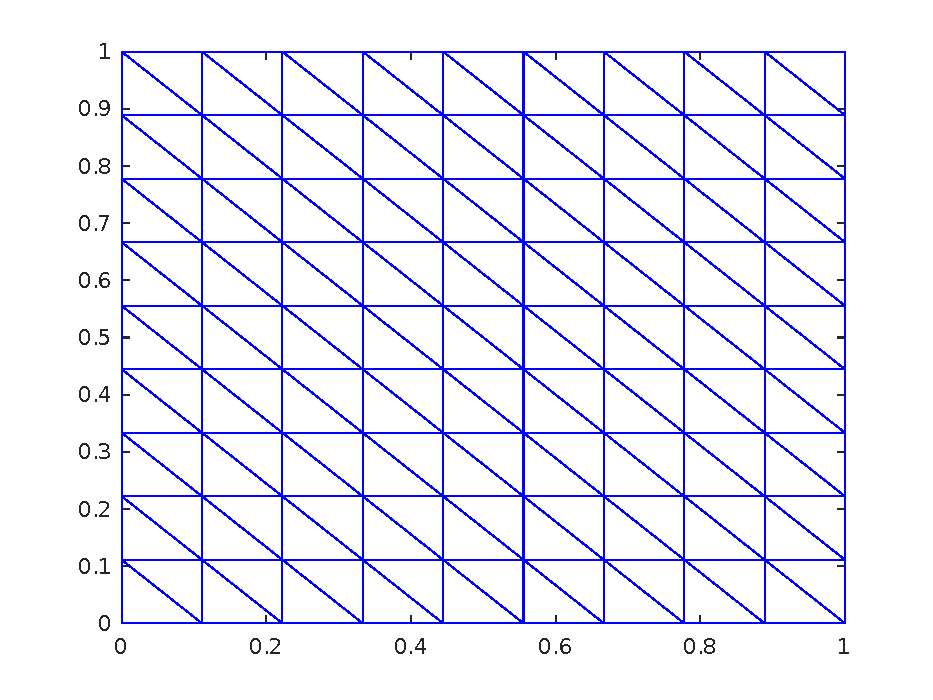
\includegraphics[width=\textwidth]{figures/basic_rect_mesh}
    \caption{A very basic meshing procedure for trivial geometries. Simply perform a Delaunay triangulation on a regular grid of points.}
    \label{fig:basic_rect_mesh}
\end{figure}

\end{document}